\chapter{Implementation}

%The implementation should look at any issues you encountered as you tried to implement your design. During the work, you might have found that elements of your design were unnecessary or overly complex, perhaps third party libraries were available that simplified some of the functions that you intended to implement. If things were easier in some areas, then how did you adapt your project to take account of your findings?

%It is more likely that things were more complex than you first thought. In particular, were there any problems or difficulties that you found during implementation that you had to address? Did such problems simply delay you or were they more significant? Your implementation might well be described in the same chapter as Problems (see below).

It is a good idea to first build a basic prototype.  Building a prototype will quickly highlight the main flaws in the initial design.  This is not the same as the intended final version and in this case is not even the same materials as I have chosen.  It does however conform the basic design but is made from much cheaper sourced components.  I already had an Arduino Uno (the basic prototyping model) from my interest int he technology before I attended university, so this was an easy component to get ym hands on quickly and is perfect for a prototype.  I had no chassis built or any materials to make one so I found a cheap and easy to assemble one online at a hobbyist electronics retailer.  This kit also included some very small DC motors with gearboxes and wheels, very convenient little package.  The Arduino alonge with the chassis kit and a small infrared sensors, a 9 volt battery and some jumper wires and a ptorotype was put together in an afternoon.
\begin{figure}[h]
\centering
        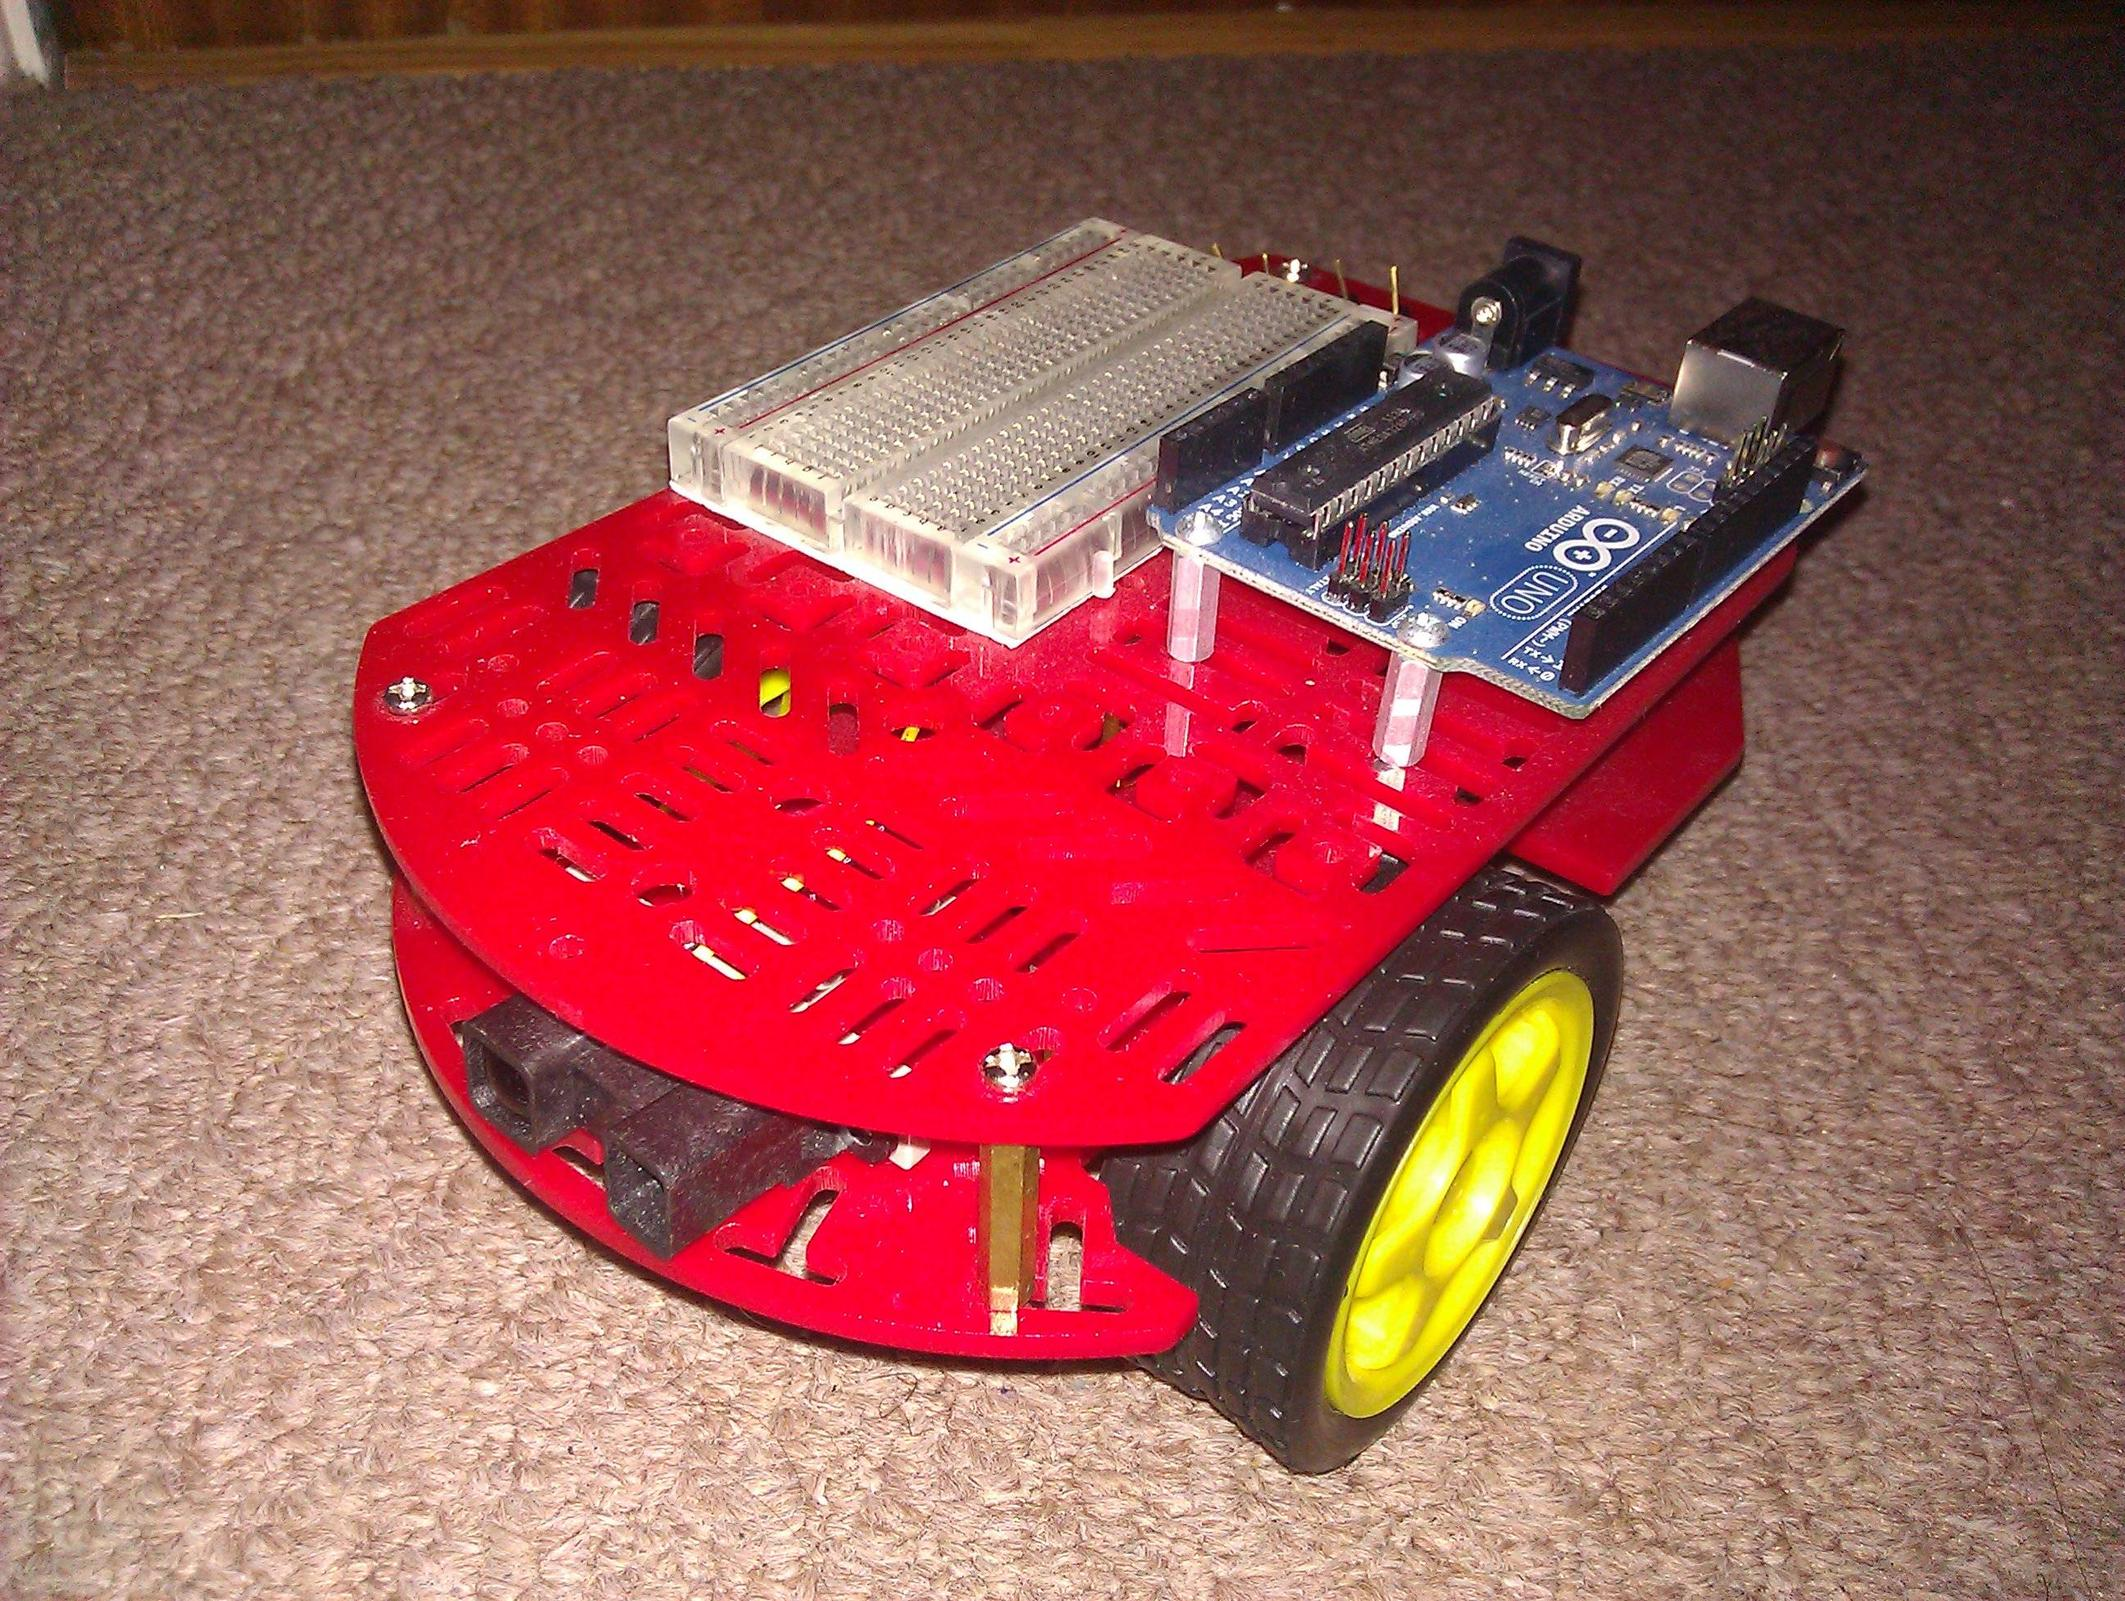
\includegraphics[width=3.0in] {Images/tria-mkI.jpg}
        \caption{Prototype mkI}
        \label{Prototype mkI}
\end{figure}

Wiring up the components was fairly easy due to there only being two motors and a single infrared sensor.  The sensor just has 3 pins, ground and possitive power pins as well as a signal pin.  This is basicly set up like a resistor, you supply power the the possitive pin, attach the ground to the ground of the system and just read the value comming back on the signal pin.  The difference between zero up to the amount of power being given to the sensor, in this case the datasheet specified 5 volts and that is what I supplied it with, gives an inidication of how far it is from an object.  With this sensor the higher value returned is actually how close the object is and the lower number indicates it is further away.  This is due to the fact that the reading recieved is indicating how intense the amount of infrared getting back to the sensor is.
\\The harder part of this was getting the motors to run safely.  The arduino I use for prototyping can only output a regulated voltage of 3.3 or 5 volts.  The motors supplied with the chassis kit do not run very well at this voltage and struggle to move on carpet.  As the supply I am using to power the Arduino is a 9 volt battery this was usfficient to run the motors at an acceptable level, the only problem is supplying this to both the Arduino and the motors.  As the microcontroller is needed to control when and how fast the motors are to turn, simply wiring the power supply directly to the motors is a bad idea as they will just spin constantly due to always having power.
\begin{figure}[h]
\centering
        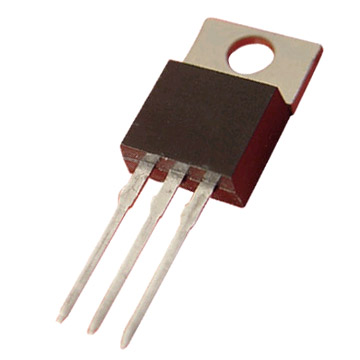
\includegraphics[width=2.0in] {Images/transistor.jpg}
        \caption{Transistor - zmescience.com}
        \label{Transistor}
\end{figure}

This could be solved using a transistor (a semi-conductor device used to switch electrical signals) by suppling it with the higher voltage, connecting it to the motor and when a signal voltage from the Arduino is recieved it switches to the higher voltage allowing the motor to turn.  This is a very handy little component which is at the core of modern day electronics, but to use it in this fashion would need a lot more complicated circuitry as to ensure that this higher voltage does not damage other components in the circuit.  Another solution would be to use a chip known as a h-bridge.
\\This chip also acts like a switch but with the addition that it can change the currents direction meaning that you can not only control when the motor is on or off but also the direction it turns without additional complex circuitry.
\begin{figure}[h]
\centering
	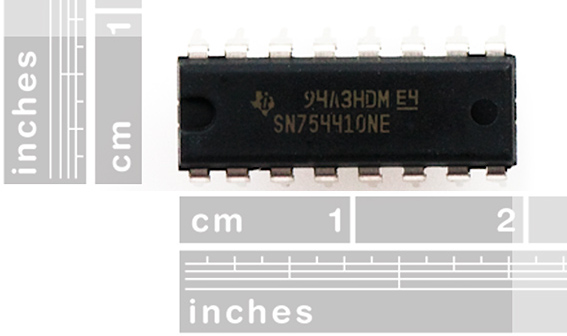
\includegraphics[width=2.0in]  {Images/h-bridge.jpg}
	\caption{H-Bridge - sparkfun.com}
	\label{H-Bridge}
\end{figure}
The h-bridge chip also has its issues, as it generates heat when high currents are passed through it so if the motors are working hard more current with be drawn and the more heat the chip will generate and possibly burn out.  There is again the issue of having no protection for the rest of the circuit.  An option that would solve this issue is a full motor driver board but the cost if these is many times the cost of the components to make the circuits myself.  For example a h-bridge chip an assortment of diodes, capacitors, resistors and transistors costs around \pounds5 while a fully built board costs around \pounds20-30.
\begin{figure}[h]
\centering
        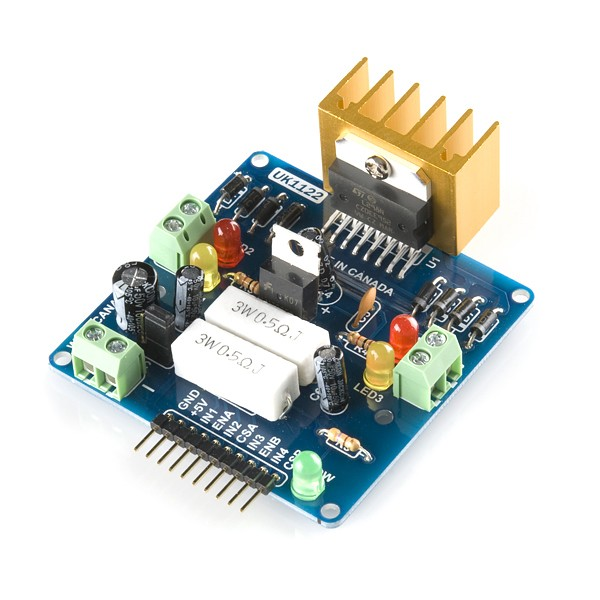
\includegraphics[width=2.0in]  {Images/motor-driver.jpg}
        \caption{Motor Driver - sparkfun.com}
        \label{Motor Driver}
\end{figure}
I decided to build a simple motor driver using the h-bridge chips, effective for a simple prototype.
\\With only a single infrared sensor the only logical place to mount it would be to have it facing directly forwards.  After writing the code to control the motors and process readings taken from the front mounted sensor the logic to test the concept is very simple.  Just check if there is something close in front and if there is just turn and check again, if there is not just keep moving forwards.
The logic looks like this:
\begin{figure}[h]
\begin{lstlisting}[basicstyle=\ttfamily]
if(sensor_range < value)
{
	motors.turn.right(45);
}else
{
	motors.move.forward(1);
}
\end{lstlisting}
\caption{Prototype Code Exert}
\label{Prototype Code Exert}
\end{figure}

